\chapter{Evaluation}

\section{Introduction}
CEP engines are used in a variety of scenarios, each of which has different requirements and settings, and that makes performance evaluation a true challenge. In fact there is not a universally agreed methodology of measurement and there are neither a reference workload, recorded from a real execution, nor a standard emulator, to generate a synthetic one.

The complexity is given by the high number of parameter that characterize the execution of the application and in particular by the different ways in which they interact.\\
In a real world scenario most of those variables are bound to the environment and very specific: the inputs are correlated one each other and together deliver a meaningful information, at the same time the rules are manually tailored to the particular task.\\
On the opposite side, during a general purpose evaluation, it is necessary to control the behavior of the inputs and the complexity of the rules, while preserving the stability of the execution.

In this chapter I will present the results of a selected number of test cases, explaining why each configuration was chosen and how it could impact on a real world application.

\section{Environment}
\begin{table}[h]
  \begin{center}
    \begin{tabular}{|c|c|}
      \hline
      Processor: 		& Intel Core i7-4770 @ 3.40GHz\\
                        & 4 Cores, 8 Threads\\ 
      \hline
      RAM size: 		& 16GB\\
      \hline
      Operating System: & Debian GNU/Linux 8.6 (jessie)\\
                        & Kernel 3.16.0-4-amd64\\
      \hline
      C++ Compiler:     & G++ 4.9.2\\
      \hline
      Rust Compiler:    & 1.14.0-nightly (2016-11-05)\\
      \hline
    \end{tabular}
    %\caption{Execution environment}
  \end{center}
\end{table}

\section{General Performances}
First of all, setting temporarily aside the introduction of static data, we will compare the previous T-Rex engine with the rewrite T-Rex2. This will show that the new implementation is indeed correct and efficient, mitigating the risk of a bias in the tests due to a poor realization. In the meantime we will gradually introduce the key points of the evaluation process and the general environment setup.

\subsection{Characteristic variables}
We start from the fundamental variables that characterize a CEP evaluation, in particular explaining their on the computation.
\begin{itemize}
\item The frequency of events and the size of predicate window are two of the most characteristic control variables and, in combination one with each other, they regulate the amount of events retained by the system. So higher frequencies and wider windows imply that more events will be associated with every predicate processor: those events have to be searched at each iteration of the system and directly concur in rules satisfaction.
\item The number of rules intuitively impact the computational requirements increasing the number of step needed to process an incoming event. However this aspect is strongly related with the number of declared event types and since the latter influence the probability of a rule being activated by the next random event. So a high number of rules composed by many different event types, may be activated just one at a time and stress the system way less than the half of the rules with fewer event declarations.
\item The number of predicates per rule and the presence of constraints on them influence the probability of a rule to be satisfied. In combination with the selection policy, measured in terms of probability of being $each$, $first$ or $last$, they determine how many new events will be generated by each rule.
\item Finally we mention the two most important output variables: the drop rate and the time of completion. The drop rate analyzes the system in a latency oriented fashion and it is measured as the percentage of discarded events: we feed the engine through a buffer queue of finite length and if it is not emptied fast enough the exceeding events are lost. On the other hand the completion time is more throughput oriented and it is obtained using an unbounded queue and waiting for the system to process every single event.
\end{itemize}

\subsection{Base rule}
As for the rule definition, the challenge is to create a model that is simple enough to predictably work under all the circumstances examined and rich enough to be interesting and customizable. We found the following rule to be representative of the different aspects we care about, while being easy to extend.
\begin{align*}
&declare\ SE_0(x:\ int)\ with\ id\ 0\\
&declare\ SE_1(x:\ int)\ with\ id\ 1\\
&declare\ \ldots\\
&declare\ SE_i(x:\ int)\ with\ id\ i\\
&declare\ CE()\ with\ id\ i+1
\end{align*}
\begin{align*}
&from\ SE_0(x == 1)\\
&and\ each\ SE_1(x == 1)\ within\ \tau_1\ from\ SE_0\\
&and\ \ldots\\
&and\ each\ SE_i(x == 1)\ within\ \tau_i\ from\ SE_{i-1}\\
&emit\ CE
\end{align*}

The rule is composed of a linear chain of simple events from $SE_0$ to $SE_i$, where every predicate has a temporal dependency with the previous one and the number of predicates can be extended at will. Each constraint is composed of a single equality to the immediate value 1, this configuration allows to simply control the match through the choice of event values. The time window is parameterized by $\tau_i$ and, while the example shows only the use of $each$ selection policy, they can be varied with a given probability.\\
Exactly $i+1$ tuples were declared, so that each one can only appear in a specific position in the rule, improving the predictability of the system.

\subsection{Workload}
\label{subsec:first-workload}
For the benchmark we configured the previous rule with $i=2$ and $\tau_i$ as a random random value uniformly distributed in the range $\tau_{avg} - 1s$ and $\tau_{avg} + 1s$.\\
The probability of choosing $each$, $first$ or $last$ selection policies was usually fixed to $100\%$ of $each$ to maximize the load of the system.\\
Regarding the rest of the system, $65$ group of $4$ event types were declared and $650$ rules were instantiated, $10$ identical for each group of events, so that every time a sequence was satisfied ten rules would fire. The events were generated uniformly across the different declarations, with all the attributes $x$ set to 1 to satisfy the constraints, and they were emitted at a tunable frequency. The number of events fed to the system was $60 * freq$, that is the quantity emitted in a minute at the given frequency. The length of the queue was bound as $freq / 10$ when measuring the drop rate and left unbound when measuring execution time.

\subsection{T-Rex and T-Rex2 comparison}
For the first comparison we set the predicates window to at an average of 10s and varied the frequencies from 600 to 4000 events per second, so that at the minimum both handle all the events, with a drop rate of 0\% and at the end of the scale most of them are lost.\\
Figure \ref{fig:trex_vs_rewrite_freq_drop} shows that the drop rate of the rewrite is lower at every frequency and similarly figure \ref{fig:trex_vs_rewrite_freq_time}, that plot execution times in second on logarithmic scale, shows that at frequencies where the engines would loose events the speed of the rewrite is almost constantly four times higher.
\begin{figure}[h]
\captionsetup{justification=centering}
\begin{minipage}{.5\textwidth}
  \centering
  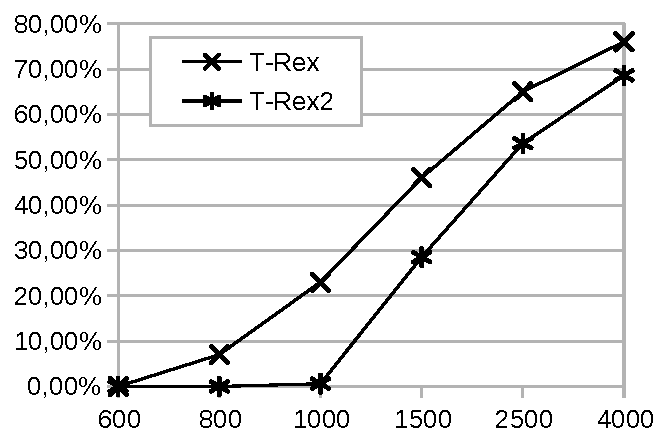
\includegraphics[width=.95\linewidth]{trex_vs_rewrite_freq_drop}
  \caption{T-Rex vs T-Rex2\\
  	Frequencies and drop}
  \label{fig:trex_vs_rewrite_freq_drop}
\end{minipage}%
\begin{minipage}{.5\textwidth}
  \centering
  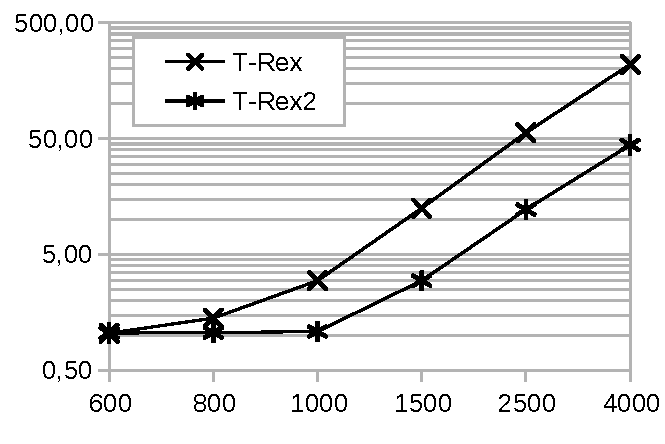
\includegraphics[width=.95\linewidth]{trex_vs_rewrite_freq_time}
  \caption{T-Rex vs T-Rex2\\
  	Frequencies and time}
  \label{fig:trex_vs_rewrite_freq_time}
\end{minipage}
\end{figure}

To better explore the domain, for the second comparison we pick a middle frequency, 1500, and vary the average windows size, in a range from 3 to 12 seconds.\\
The results, shown in figure \ref{fig:trex_vs_rewrite_win_drop} and \ref{fig:trex_vs_rewrite_win_time}, are noticeably similar to the first measurement and confirm the performance gain.\\
We can also observe how in both the test case the drop rate and the corresponding execution time are closely correlated and most of the time it is possible to switch from one to the other without loosing the qualitative interpretation.
% TODO maybe add the observation that
% they correlate exponentially: that is likely to happen since the system, discarding packages, reduces event retention and a 10\% global reduction, translates in a 10\% at each step of the pattern composition
\begin{figure}[h]
\captionsetup{justification=centering}
\begin{minipage}{.5\textwidth}
  \centering
  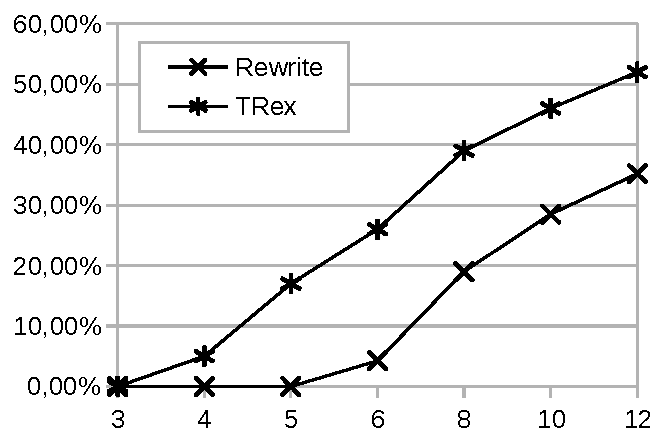
\includegraphics[width=.95\linewidth]{trex_vs_rewrite_win_drop}
  \caption{T-Rex vs T-Rex2\\
  	Windows and drop}
  \label{fig:trex_vs_rewrite_win_drop}
\end{minipage}%
\begin{minipage}{.5\textwidth}
  \centering
  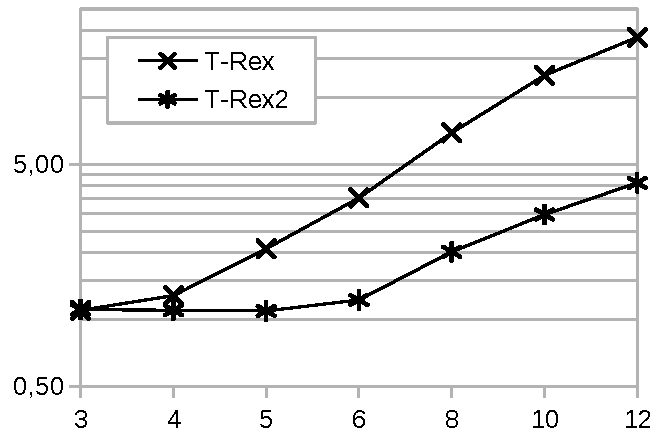
\includegraphics[width=.95\linewidth]{trex_vs_rewrite_win_time}
  \caption{T-Rex vs T-Rex2\\
  	Windows and time}
  \label{fig:trex_vs_rewrite_win_time}
\end{minipage}
\end{figure}

The results demonstrate the efficiency of T-Rex2, with improvements that can be considered beyond the expectations, considering that the rewrite closely followed the architecture of its predecessor. The most likely and relevant motivation is a slightly improved parallelism that take advantage of all the available processing units: they both had 8 workers threads (plus few other to deal with coordination and event publishing), but the old implementation distribute the jobs statically using rule ids, while the rewrite allocate them dynamically with a thread pool.\\

\section{Static data and Cache}
In this section we are going to explain how the execution must be adapted to evaluate the interaction between events and persistent data and to test the performance gains obtained from the cache.

\subsection{Additional variables}
We must refine the domain of the problem, since the new expressivity inevitably causes the expansion of the control variables with the one needed to describe the properties of the database and the cache layer.\\
In particular a database is a complex technology and have plenty of settings and characteristic, but the fundamental ones are: the number of rows, the number of columns, the distribution of the values, the latency of the connection and the presence of indexes. While the integration into the CEP execution is characterized by the selection policy, the constraints on the values, the number of results and the frequency of invocation.\\
As for the cache, there is the choice of the algorithm among the many presented, the size in terms of memory occupation and finally the possibility to share the storage or split it among the different users. Moreover there are environmental factors that influence the results like the domain and the probabilistic distribution of the values. Finally miss rate and hit and miss time are the characteristic metrics of performance.

\subsection{Rule adaptation}
The previous TESLA rule was kept as a template and extended with a static predicate with the following configuration:
\begin{align*}
&declare\ SE_0(x:\ int)\ with\ id\ 0\\
&declare\ SE_1(x:\ int)\ with\ id\ 1\\
&declare\ \ldots\\
&declare\ SE_i(x:\ int,\ y:\ int,\ z:\ int)\ with\ id\ i\\
&declare\ SE_{i+1}(col_0:\ int,\ \ldots,\ col_j:\ int)\ with\ id\ i+1\\
&declare\ fact\ SD(col_0:\ int,\ \ldots,\ col_j:\ int)\ with\ id\ i+2\\
&declare\ CE()\ with\ id\ i+3
\end{align*}
\begin{align*}
&from\ SE_0(x == 1)\\
&and\ each\ SE_1(x == 1)\ within\ \tau_1\ from\ SE_0\\
&and\ \ldots\\
&and\ each\ SE_i[\$p_1 = y,\ \$p_2 = z](x == 1)\ within\ \tau_i\ from\ SE_{i-1}\\
&and\ each\ SD[\$c_0 = col_0](col_1 >= \$p_1,\ col_1 < \$p_2)\\
&emit\ CE(x = \$c_0)
\end{align*}
There is a new declaration $SD$ that describes the static data collection and each of its attributes is mapped to a column of the table.\\
The event $SE_i$ acquire a special role, it has a second and third attribute, that are referenced in the static predicate and they work as lower and upper bound, controlling the result of the query.\\
Another declaration was introduced, $SE_{i+1}$, that, as we will see, can be used as a replacement of $SD$ whenever we want to reduce the access to the DB while keeping the same level of produced events.\\
Finally it is possible, through a configuration, to add a parametric dependency between the static predicate and other predicates in the rule: this allow to expand the domain of the cache key stressing the cache algorithms.

\subsection{Workload}
\label{sec:second-workload}
% database creation, database random data, extension of the rule (last predicate), 1000 rules 100 declarations, highly frequent and dense, now focused on each sel policy
First of all, a database table is created with 2 columns (an incremental index and a numerical payload) and populated with a given number of rows. In particular, for each entry the aforementioned payload is randomly generated in a range between $-1 / 2 * \#rows$ and $+1 / 2 * \#rows$: having a uniform distribution of values, but in a non sequential order, helps to avoid possible bias in term of DBMS architecture or file read.\\
The declaration were changed to 100 groups of 5, plus one single declaration for the database table. The rule defined are 1000, preserving the ratio of 10 identical rule for each declaration group. Database indexing can be switched on or off.\\
During the event generation, $SE_i.y$ (the second attribute of the events of type $SE_i$) is set to a random value, sampled from a selectable probabilistic distribution, while $SE_i.z$ is set as $SE_i.y + \Delta$, so that they act properly as lower and upper bound. Where $\Delta$ is generated pseudo-randomly with an average of 10.\\
What is not mentioned here is unchanged from the previous definition of the workload in section \ref{subsec:first-workload}.

\subsection{Table simulation and database}
Even without a native support for DBMSs, it was already possible to emulate the access to a persistent data collection, as we recall from section \ref{sec:intro-lang-extension}. So it seems appropriate to verify the integration with SQLite to be consistently faster than preexisting alternative.

So, to define two executions with the very same semantic, we applied the algorithm for DB population to produce events with the same payload of the corresponding table and we emitted all of them at the beginning of the execution. At the same time we adapted the static predicate in each rule extract the same data from the simulated event stream (using an unlimited window, to have the data available at any time).

\begin{figure}[h]
  \centering
  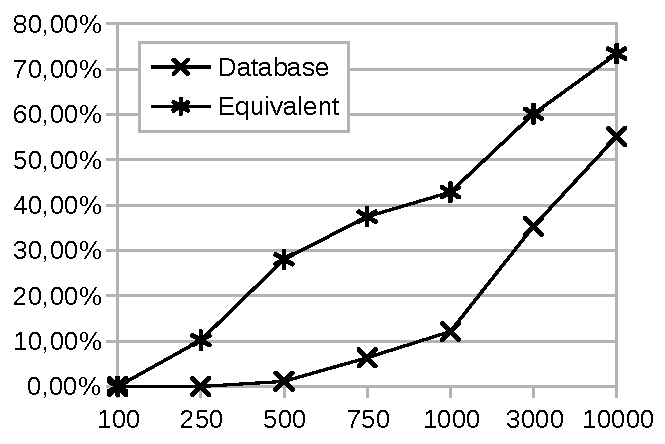
\includegraphics[width=.6\textwidth]{equiv_vs_db_800r_drop}
  \caption{Database vs simulation}
  \label{fig:equiv_vs_db_800r_drop}
\end{figure}

We execute the programs with a small window of 2s average and low frequency of 800 events per second, varying the number of static data entries from 100 to 10000. As we can see from figure \ref{fig:equiv_vs_db_800r_drop}, the table simulation fully handle the load only with a very small collection and performances rapidly deteriorate as soon the number of static entries grow. On the other hand, T-Rex2 does not lose events even with the highest configuration considered. It is worth noting that, actually, thanks to the benefits of the database index, the performance of T-Rex2 are virtually not influenced by the size of the table (tested up to 10 million rows).
% TODO add second test with high performances

The results show that a native support is clearly an important improvement to the previous possibilities, but at the same time they give us little information about the limits of T-Rex2.

\subsection{Performances contextualization}
In the following benchmark we contextualize the measures collected through a comparison of the results of three different configuration that have the same rate of event production, meaning that given the same number of input events they will output a similar number of complex events.\\
Two out of thee different competitors share exactly the same workload described in section \ref{sec:second-workload}, one uses the dummy cache and the other uses the perfect one. The remaining execution does not have static predicates and is constructed in this way: each predicate of type $SD$ is replaced with one of type $SE_{i+1}$, with no constraints and unlimited window, and then events of type $SE_{i+1}$ are generated in the same number as the average length of the database result set (10 in this case). In this way the behavior of the system is closely simulated.\\
The test is run with an average predicate window of 6 seconds, 1 million of table rows (where used) and a frequency of events that vary from 600 to 4000 events per second.

\begin{figure}[h]
  \centering
  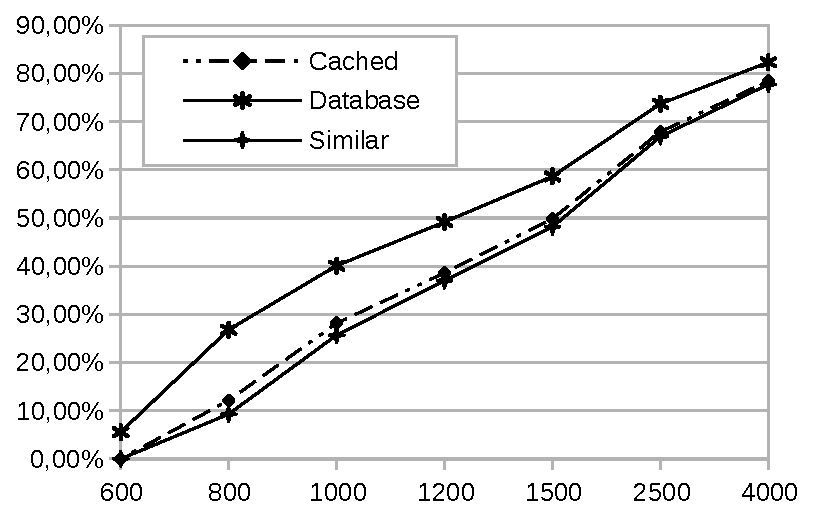
\includegraphics[width=.85\textwidth]{db_or_not_db_cached_drop}
  \caption{Perfect cache - Frequency and Drop}
  \label{fig:db_or_not_db_cached_drop}
\end{figure}

The results in figure \ref{fig:db_or_not_db_cached_drop} shows that that T-Rex2 integrated with SQLite in combination with a perfect cache (dashed line in the middle) can almost keep up with an execution that does not require access to the database (lowest line), loosing just around $2\%$ of events more than the competitor. At the same time the execution with the dummy cache draw a lower limit for the worst case performance: so, even in presence of non cache-friendly data or using less performing caches, the system is still capable of handling a remarkable load, likely enough to satisfy the requirements of many real applications.

\subsection{Cache algorithms}
% LRU_SIZE vs GDFS vs COLLISION (not a big difference, why?)
Now that we have defined some term of comparison and showed the results of the best and worst cache, in the following paragraphs we are going to analyze the performance of all the cache algorithms presented in section \ref{sec:cache-impl} to see how they compare one with the others.

For the execution we set a frequency of 2000 event per second and 2 seconds window, with the event payload sampled from a normal distribution $\mathcal{N}(\mu = 0,\ \sigma = 30)$ and making the static query dependent from the last two predicates (expanding the query parameterization space, making harder to cache enough values). Then we vary the cache size, measured as the number of the rows contained in each cache object, from 500 to 6000.\\
We first analyze the miss rate of each algorithm, see figure \ref{fig:cache_showdown_miss}, and then compare it to the corresponding drop rate to evaluate the impact on the global execution, see figure \ref{fig:cache_showdown_drop}.

\begin{figure}[h]
  \centering
  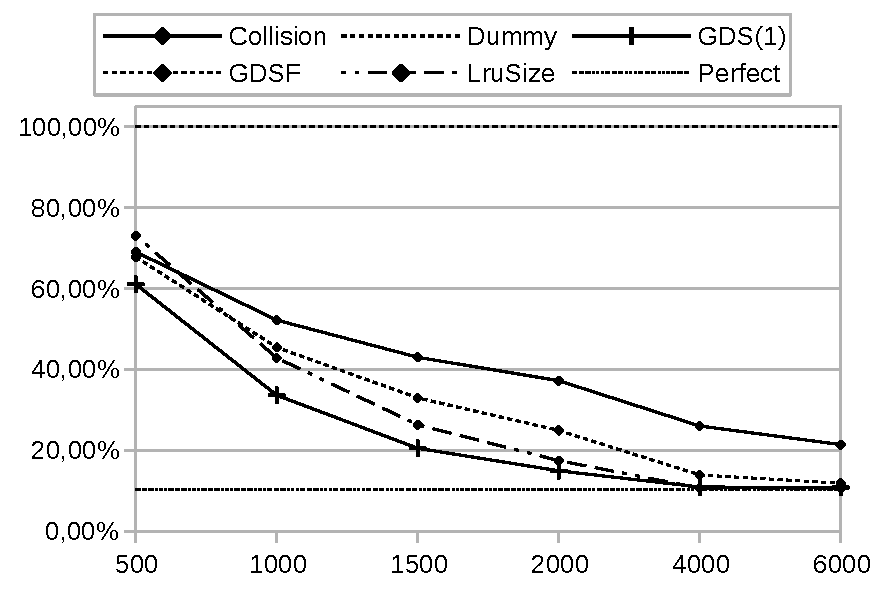
\includegraphics[width=.8\textwidth]{cache_showdown_miss}
  \caption{Cache comparison - Frequency and Miss}
  \label{fig:cache_showdown_miss}
\end{figure}
\begin{figure}[h]
  \centering
  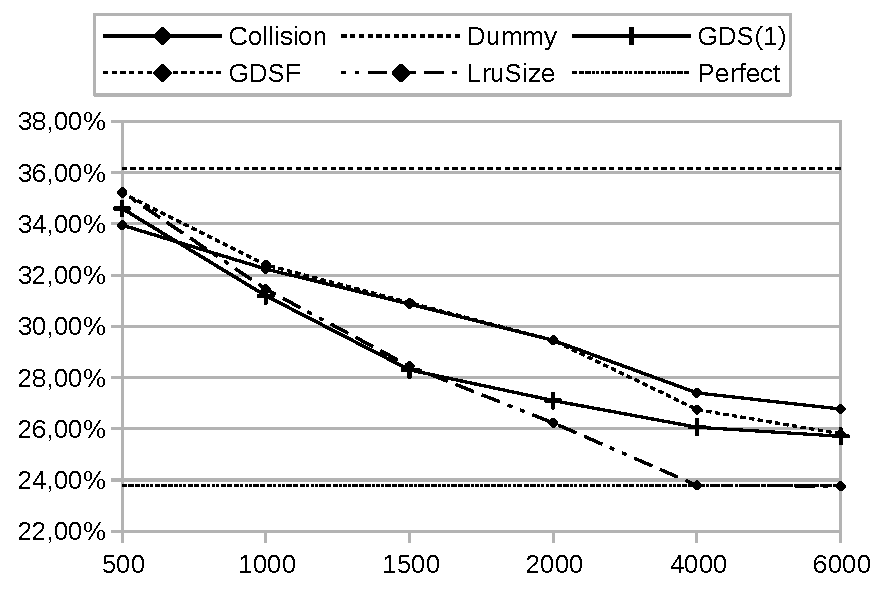
\includegraphics[width=.8\textwidth]{cache_showdown_drop}
  \caption{Cache comparison - Frequency and Drop}
  \label{fig:cache_showdown_drop}
\end{figure}

The dummy cache once again shows the worst case performances with $100\%$ miss rate. While the perfect cache sets the upper limit for the maximum efficiency achievable, with a $10\%$ of miss rate. They are shown on the charts as a horizontal line respectively at the top and at the bottom of the plots. At the end of the execution the perfect cache contained about 12000 entries, that is the size of the key space.\\
The collision cache, that is built on a very basic replacement policy, had a poor performance and was exceeded by every other algorithm.\\
However it was unexpected to see the GDSF cache, that is the de facto standard and champion in HTTP caching, to be clearly left behind in the comparison. My intuition is that its measure of frequency does not work well with the repeated access patterns of a CEP engine would require a more precise tuning.\\
The second best is the LRU-size, that proves itself to be a good allround solution and the first choice for any caching purpose. The winner of the comparison is the GDS(1) cache, that choosing smaller entries is able to maximize the memory usage. We can also notice, that both the top two algorithms reach the level of optimality of the perfect cache with a size between 2000 and 4000 entries, that means 3 to 6 time less than the actual key space.

Comparing the results with the plot of system wide performances, we show that the sole minimization of the miss rate it is not sufficient affect the global execution. The most notable example is how GDS(1), champion of the previous category, fails to keep up with LRU. The phenomenon is explained by the difference in term of hit time: in fact GDS(1) does have more hits (between $5\%$ and $10\%$ more), but with a cost of almost the double of the LRU ($\sim 1200 \nu s$ compared to $\sim 650 \nu s$ of access time). The reason behind this slow down is likely due to the suboptimal GDS(1) implementation.

\subsection{Shared or per predicate}
When the cache is allocated as a single storage accessed by different predicates, if they request similar data they will share the space and the cache loading cost. Also if there is some process that has more benefits from caching, an advanced algorithm could reward it with more space in memory. However there is always the risk that a single component would hog the entire space, filling it with garbage and degrading the system wide performance.\\
A cache per predicate, instead, would be much smaller, but it could better adapt to the specific pattern or distribution of the data.\\
However we found out to be another the most relevant factor decision: sharing the cache across multiple threads require constant synchronization. In the implementation the cache is wrapped with a mutex that soon became the bottleneck of the entire parallelization.

\subsection{Data distribution}
First of all we need to clarify that having a discrete and not too dense domain of values is a fundamental requirement, otherwise even in the smallest range there would be to many elements to hope for a reasonable match in the cache. So for example floating point numbers usually not adapt to take part to the cache key.\\
The effectiveness of a cache is based on assumptions on the processed data, for example time locality, meaning that a value requested recently is likely to be requested again. Each assumption may fit better or worse depending from the actual data distribution.

The system was built to offer a choice about the distribution of the input event values. So it is possible to experimented with gaussian, exponential and uniform distributions tuning the parameters to spread or narrow the range of the samples.\\
However we found out that this is only partially relevant, in fact there is a limit to the variability that can be introduced by a single event: because of the nature of the system, only a restricted number of events is queued in a processor and that is the maximum expression of the distribution. Conversely sequences of evaluation are executed repeatedly and the same data is requested many time during a single system iteration, so the benefit of the cache prevail over any possible distribution.\\
The situation changes when we make the static predicate dependent from more than one event at a time: in this case the probability distributions combine with each other and generate a wider and more diverse output, challenging the capacity of the cache.

%\section{Additional factors}
%\subsection{Event selection policy}
% EACH vs FIRST/LAST
%\subsection{Percentage of static predicates}
% PERCENTAGE OF STATIC PREDICATES and SATURATION FREQUENCY
%\subsection{Parallelism}
% N OF CORES
